\chapter{Геометрия твердых тел}
\section{Геометрические примитивы}
Описание движения тела полностью абстрагировано от его формы
или, как принято выражаться, геометрии --- это очень важно
уяснить для понимания внутренней архитектуры физического
движка.

Основными геометрическими примитивами используемыми в физических движках являются:
\begin{itemize}
 \item  луч, 
 \item  плоскость,
 \item  полигон,
 \item  сфера,
 \item  треугольник
 \end{itemize}
Для реализации более сложных геометрических тел используется композиция тел представленных выше.

Рассмотрим более подробно один основных из геометрических примитивов --- сферу.
Сфера может быть описана в пространстве положением своего геометрического цента(он же является и центром масс)
и радиуса. Таким образом для описания сферы достаточно 4 компонент : вектора положения центра сферы( 3 компоненты) и радиуса сферы.

%TODO Рассмотреть большее количество геометрически примитивов

\section{Контакт геометрических тел}
Реализации твердого тела и геометрического объекта как правило раздельны --- геометрия тела играет роль только в
процессе обнаружения столкновений, рассматриваемый ниже.

Модули обнаружения столкновений (\textit{collision detection}) и реагирования на столкновения (\textit{collision responce}) представляют 
собой ключевые компоненты любого физического движка. Именно они в процессе симуляции осуществляют главную нагрузку на
процессор, и именно от них требуется максимальная точность.

\subsection{Обнаружение столкновений}
Методы обнаружения столкновений подразделяются на две категории: статические и динамические. В первом случае
движение тел рассматривается как последовательность «квантовых скачков» --- проверка на пересечение двух геометрий
производится в промежутках между скачками, как если бы объекты в этом время не двигались (то есть, имели нулевые
скорости). Основным допущением этого метода является временная когерентность системы --- предполагается, что тела
обладают небольшими скоростями, и их позиции не меняются слишком резко с течением времени. Иными словами,
статическое обнаружение столкновений плохо подходит для моделирования, например, пушки, стреляющей в бетонную
стену: за шаг времени ($\Delta{t}$) снаряд пройдет расстояние, значительно превышающее толщину стены, и, следовательно,
попросту пролетит сквозь нее --- статическая проверка это столкновение не обнаружит.

Динамическое обнаружение столкновений\cite{Ericson} использует другой метод, при котором учитывается скорость тела --- движок
предсказывает, какое положение в пространстве займет объект на следующем шаге времени, если будет двигаться с той же
скоростью. Фактически, делается проверка на пересечение отрезка, представляющего собой траекторию движения тела, с
препятствием --- вычисляется точка, в которой тело столкнется с этим препятствием, и на основании этой информации движок
делает соответствующие корректировки. К сожалению, динамический метод довольно сложен (особенно для
нетривиальных геометрий) и, в целом, плохо адаптирован для динамики как таковой --- он чаще используется в кинематике.
Поэтому далее будет рассматриваться статический метода --- он, при всех его недостатках, хорошо себя оправдывает в
большинстве физических ситуаций.

В физическом движке функция проверки столкновения между двумя объектами должна давать на выходе следующую
информацию:
\begin{itemize}
  \item точка контакта
  \item вектор нормали к поверхности столкновения в этой точке (нормаль контакта)
  \item глубина взаимного проникновения объектов
\end{itemize}

\begin{figure}[ht!]
\begin{center}
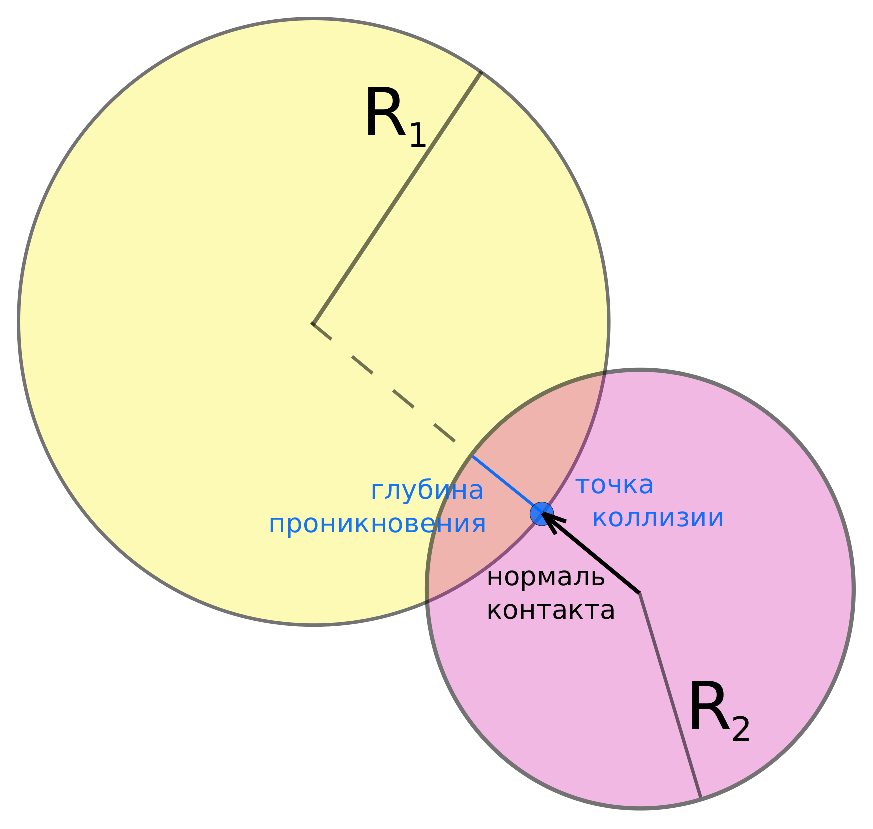
\includegraphics[scale=0.45]{./Geometry/SphereCollision.eps} \\
\caption{Контакт двух сфер}\label{SphereCollision} 
\end{center}
\end{figure}
Эти три свойства, вкупе со ссылками на столкнувшиеся тела, дают новую сущность --- контакт. Соответственно,
процесс обнаружения столкновений в терминологии физического движка также называют генерированием
контактов (\textit{contact generation}). В сложных движках на одно столкновение между двумя телами приходится несколько
контактов --- так называемый \textit{contact manifold}. Далее будет рассматриваться простейший случай --- столкновение сфер, где будет
достаточно одного контакта на пару столкнувшихся тел.

Рассмотрим одно очевидным свойство. Если сумма радиусов двух сфер превышает расстояние между их центрами, следовательно, сферы пересекаются.
При этом нормаль столкновения --- это нормированный вектор от центра второй сферы в сторону центра первой,
точка столкновения --- экстремальная точка на поверхности второй сферы в направлении этого вектора, а глубина взаимного
проникновения --- разница между суммой радиусов и расстоянием (см. рисунок \ref{SphereCollision}). % здесь ссылка возможно 
% и не нужна, вставил для пробы

Таким образом можно легко обнаружить столкновение таких двух примитивов как сферы.
\subsection{Реагирование на столкновение}
Получив необходимую информацию о контакте(точку контакта, нормаль контакта и глубину проникновения), модулю реагирования
на столкновения необходимо скоординировать скорости тел таким образом, чтобы тела перестали пересекаться и проникать друг в друга.  

При моделировании используются алгоритм отличный от реального поведения: объекты выталкиваются вдоль вектора нормали на величину,
равную половине глубины взаимопроникновения:

\begin{equation}
\mathbf{x} = \frac{1}{2}\mathbf{x}_0 + d\mathbf{n}
\end{equation}
\begin{eqrem}
$\mathbf{x}_0$ --- точка контакта,

$d$ --- глубина взаимопроникновения,

$\mathbf{n}$ --- вектор нормали контакта.
\end{eqrem}

Первый объект выталкивается вдоль $+\mathbf{n}$, а второй --- вдоль $-\mathbf{n}$ (вектор нормали контакта указывает от второго тела к первому).

Эту операцию называют также корректировкой позиций (\textit{position correction}). Но такой подход нестабилен, кроме того,
необходимо учитывать массы тел и, следовательно, импульс.

Импульс --- это векторная величина, мера механического движения тела. Вращательным аналогом импульса является момент импульса.
\begin{equation}
\mathbf{L} = \mathbf{r}\times\mathbf{p}
\end{equation}
\begin{eqrem}
$\mathbf{p}$ --- линейный импульс,

$\mathbf{r}$ --- радиус-вектор (точка, к которой приложен линейный импульс).
\end{eqrem}


Далее будет рассмотрен один из методов разрешения контакта более точно моделирующий реальность с физической точки зрения.

\section{Разрешение контакта}

Продолжим рассмотрение частного случая - контакта двух шаров. Пусть скорость первого шара равна $\mathbf{v}_1$, скорость второго - $\mathbf{v}_2$.
Тогда относительную скорость$\mathbf{v}_{rel}$, без учета вращения, в точке контакта $\mathbf{x}_0$  можно рассмотреть, например, в системе отсчета второго шара,
она будет равна:
\begin{equation}
\mathbf{v_{rel}} = \mathbf{v_1} - \mathbf{v_2}
\end{equation}

Из курса механики известно, что если тело вращается вокруг центра масс $\mathbf{x}$  с угловой скоростью $\mathbf{\omega}$,
то скорость его точки $\mathbf{p}$ можно выразить как
\begin{equation}
\mathbf{v_p} = (\mathbf{p} - \mathbf{x}) \times \mathbf{\omega} 
\end{equation}

Таким образом ограниченной степени свободы с учетом угловой скорости принимает вид:
\begin{equation}
\mathbf{v_{rel}} = \mathbf{v_1} + (\mathbf{p} - \mathbf{x_1}) \times \mathbf{\omega_{1}} -  \mathbf{v_2} - (\mathbf{p} - \mathbf{x_2}) \times \mathbf{\omega_{2}}
\end{equation}

Выразим проекцию относительной скорости $\mathbf{v_{rel}}$ на нормаль контакта $\mathbf{n}$, она определяется скалярным произведением:
\begin{equation}
v_{proj} = \mathbf{v_{rel}} \mathbf{n}
\end{equation}

Если потребовать: 
\begin{equation}
v_{proj} = 0
\end{equation}
то тем самым будет ограничена одна степень свободы системы --- движение тел вдоль нормали контакта. Важно понимать,
что, удовлетворение этого требования, лишь запрещает контактирующим телам проникать глубже друг в друга, никак не разрешая коллизию в случае,
если тела пересеклись.

Преобразуем объединив в одно выражение:
\begin{equation}
    v_{proj} = \mathbf{v_1} \mathbf{n} + (\mathbf{p} - \mathbf{x_1}) \times \mathbf{\omega_{1}} \mathbf{n} 
    -  \mathbf{v_2} \mathbf{n} - (\mathbf{p} - \mathbf{x_2}) \times \mathbf{\omega_{2}} \mathbf{n}
\end{equation}

Применяя формулу векторного преобразования:
\begin{equation}
\mathbf{a} \times \mathbf{b} \mathbf{c} = \mathbf{c} \times \mathbf{a} \mathbf{b} 
\end{equation}

преобразуя, получаем: 
\begin{equation}
    v_{proj} = \mathbf{n} \mathbf{v_1} + \mathbf{n} \times (\mathbf{p} - \mathbf{x_1}) \mathbf{\omega_{1}} 
    -  \mathbf{n} \mathbf{v_2} - \mathbf{n} \times (\mathbf{p} - \mathbf{x_2}) \mathbf{\omega_{2}}
\end{equation}

Эту формулу можно переписать в виде:
\begin{equation}
 \mathbf{n_1} = \mathbf{n} 
\end{equation}
\begin{equation}
 \mathbf{w_{1}} =  \mathbf{n} \times  (\mathbf{p} - \mathbf{x_1})
 \end{equation} 
\begin{equation}
 \mathbf{n_2} = -\mathbf{n}
 \end{equation} 
\begin{equation}
 \mathbf{w_{2}} = -(\mathbf{n} \times (\mathbf{p} - \mathbf{x_2})) 
\end{equation}

Тогда уравнение для $\mathbf{v_{proj}}$ примет вид:
\begin{equation}
 \mathbf{v_{proj}} = \mathbf{n_{1}} \mathbf{v_{1}} + \mathbf{w_{1}} \mathbf{\omega_{1}}
		 + \mathbf{n_2} \mathbf{v_{2}} + \mathbf{w_{2}} \mathbf{\omega_{2}}
\end{equation}

Откуда можно заключить, что ограничение, вносимое в систему из двух тел контактом, можно описать четырьмя векторами: $\mathbf{n_1}$, $\mathbf{w_1}$,
$\mathbf{n_2}$, $\mathbf{w_2}$.
Следует отметить, что записанные подряд координаты этих векторов образуют строку Матрицы Якоби
\begin{equation}
    \mathrm{J} = 
    \begin{pmatrix} 
     \mathbf{n_1} \mathbf{w_1} \mathbf{n_2} \mathbf{w_2}
     \end{pmatrix}
\end{equation}

и ограничение можно описать как
\begin{equation}
 \mathrm{J} \mathbf{v_{rel}} = 0
\end{equation}
\begin{eqrem}
 $\mathbf{v_{rel}}$ -- вектор обобщенных скоростей: 
 
 $\mathbf{v_{rel}}$ = 
 $\begin{pmatrix} 
     \mathbf{v_1} \mathbf{\omega_{1}} \mathbf{v_2} \mathbf{\omega_{2}}
  \end{pmatrix}$
\end{eqrem}

\subsection{Метод \textit{Sequential Impulses}}
Остается понять, как можно удовлетворить условию $v_{proj}$ = 0.

Взаимодействие столкнувшихся тел осуществляется передачей импульса в направлении нормали контакта $\mathbf{n}$
некоторой амплитуды $\lambda$ к точке контакта $x_0$ к первому телу и такого же импульса противоположенного направления второму телу.
Другими словами, тела при столкновении обмениваются импульсом  $\lambda \mathbf{n}$.

Таким образом решение поставленной задачи можно свести к нахождению $\lambda$

Рассмотрим, как изменится линейная и угловая скорость тела, если приложить к его точке $\mathbf{x_0}$ импульс в направлении нормали $\mathbf{n}$ и 
модулем $\lambda$: 

линейная составляющая высчитывается просто: делением вектора импульса на массу тела.
\begin{equation}
   \mathbf{v_{res}} = \mathbf{v} + \frac{\lambda \mathbf{n}}{m};
\end{equation}
\begin{eqrem}
$\mathbf{v_{res}}$ --- скорость после коллизии,

$\mathbf{v}$ --- вектор скорости тела
\end{eqrem}

Для вычисления угловой составляющей воспользуемся формулой:
\begin{equation}
\mathbf{\omega_{res}} = \mathbf{\omega} + ((\lambda \mathbf{n}) \times (\mathbf{p} - \mathbf{x})) \mathbf{I ^{-1}}
\end{equation}

\begin{eqrem}
$\mathbf{\omega_{res}}$ --- угловая скорость после коллизии,

$\mathbf{\omega}$ --- вектор угловой скорости тела,

$\mathbf{p}$ --- точка контакта,

$\mathbf{x}$ --- центр масс тела,

$\mathbf{I}$ --- тензор инерции
\end{eqrem}

Заметим, что изменения линейной и угловой скоростей можно выразить через уже найденные $\mathbf{n_1}$, $\mathbf{w_1}$,
$\mathbf{n_2}$, $\mathbf{w_2}$:

\begin{equation} 
v_{proj} =
      \mathbf{n_1} (\mathbf{v_1} + \frac{\lambda \mathbf{n_1}}{m_1} ) 
    + \mathbf{w_1} (\mathbf{\omega_{1}} + \lambda \mathbf{w_1}{I_1}^{-1})
    + \mathbf{n_2} (\mathbf{v_2} + \frac{\lambda \mathbf{n_2}}{m_2} ) 
    + \mathbf{w_2} (\mathbf{\omega_{2}} + \lambda \mathbf{w_2}{I_2}^{-1})
\end{equation}

Преобразуем, получаем:

\begin{equation} 
v_{proj} = \mathbf{n_1} \mathbf{v_1} + \mathbf{n_2} \mathbf{v_2}
         + \mathbf{w_1} \mathbf{\omega_{1}} + \mathbf{w_2} \mathbf{\omega_{2}}
         + \frac{\lambda \mathbf{n_1} \mathbf{n_2}}{m_1} + \mathbf{w_1} \mathbf{w_1} {I_1}^{-1} 
	 + \frac{\mathbf{n_1} \mathbf{n_2}}{m_2} + \lambda \mathbf{w_2} \mathbf{w_2} {I_2}^{-1} 
\end{equation}


Как было сказано выше, контакт считается решенным, если $\mathbf{v_{proj}}$ обращается в ноль. Получаем уравнение:

\begin{equation} 
  a = \mathbf{n_1} \mathbf{v_1} + \mathbf{n_2} \mathbf{v_2}
    + \mathbf{w_1} \mathbf{\omega_{1}}
    + \mathbf{w_2} \mathbf{\omega_{2}}
\end{equation}

\begin{equation} 
  b = \frac{\mathbf{n_1} \mathbf{n_1} }{m_1} 
    + \mathbf{w_1} \mathbf{w_1} {I_1}^{-1}
    + \frac{\mathbf{n2} \mathbf{n2} }{m_2} 
    + \mathbf{w_2} \mathbf{w_2} {I_{2}}^{-1}
\end{equation} 

\begin{equation} 
  a + \lambda b  = 0;
\end{equation} 

Очевидным решение является $\mathbf{\lambda} = -\frac{a}{b}$. Таким образом найден импульс, 
которым обмениваются тела при введении ограничения степени свободы ($\mathbf{n_1}$, $\mathbf{w_1}$, $\mathbf{n_2}$, $\mathbf{w_2}$). 


Данный метод обладает одним недостатком: при большом количестве ограничений придется решать систему уравнений, чтобы удовлетворить всем ограничениям
одновременно. Поскольку, большинство алгоритмов для решения систем линейных уравнений работают за $O(n^{3})$, такой применяется редко. 

Вместо него применяются итеративные методы, постепенно приближающие решение к более точному.
Если решать полученную систему уравнений одним из таких методов, называемых \textit{Projected Gauss-Seidel Solver (PGS) },
то последовательность производимых при этом действий математически эквивалентна последовательному решению коллизий, как описывалось выше.
Этот подход широко распространен и называется \textit{Sequential Impulses}.

Суть метода в последовательном решении ограничения за ограничением вместо решения системы ограничений.
Полученный результат будет сходиться к результату, как если бы их решали в системе.

\subsubsection{Случай упругого соударения}
Выше рассматривался случай, когда контакт считался решенным, если относительная скорость тел в проекции на нормаль контакта равняется нулю,
то есть, другими словами, случай неупругого соударения.
Алгоритм нетрудно модифицировать на случай упругого соударения. Введем коэффициент отскока $bounce$,
который принимает значения от 0 до 1, при этом случаю абсолютно неупругого соударения соответствует $bounce$ = 0, случаю абсолютно упругого - $bounce$ = 1.

Ранее было показано, чему будет равняться проекция скорости $\mathbf{v_{proj}}$,
если тела обменяются через данный контакт импульсом с модулем $\lambda$ (2.21).

Если в случае с абсолютно неупругим соударением стояло условие $\mathbf{v_{proj}}$ = 0, то изменив условие следующим образом:
\begin{equation}
\mathbf{v_{proj}}= -bounce{v_{init}}
\end{equation}
\begin{eqrem}
$v_{init}$ --- величина, равная:

  $v_{init}$  = $\mathbf{n_1}\mathbf{v_1}$ + $\mathbf{w_1}\mathbf{\omega_{1}}$
	      + $\mathbf{n_2}\mathbf{v_2}$ + $\mathbf{w_2}\mathbf{\omega_{2}}$
\end{eqrem}

Таким образом можно промоделировать соударение с разной степенью упругости.